\documentclass[13pt,a4paper]{article}
\usepackage[utf8]{inputenc}
\usepackage[russian]{babel}
\usepackage[OT1]{fontenc}
\usepackage{amsmath}
\usepackage{amsfonts}
\usepackage{amssymb}
\usepackage{graphicx}
\usepackage[left=2cm,right=2cm,top=2cm,bottom=2cm]{geometry}
\usepackage{calc}
\usepackage{wrapfig}
\usepackage{setspace}
\usepackage{indentfirst}
\usepackage{subfigure}


\title{
1.4.5.

Изучение колебаний струны
}

\author{Семёнов Андрей Б02-016}
\date{25 февраля 2021г.}
\begin{document}

\maketitle
\newpage

\textbf{Цель работы:} изучение поперечных стоячих волн на струне; определение собственных частот колебаний струны;
исследование зависимости скорости распространения поперечных волн на струне в зависимости от её натяжения.

\textbf{В работе используются:} закрепленная на станине стальная струна, набор грузов,электромагнитные датчики, звуковой генератор, двухканальный осциллограф, частотомер

\section{Теоретические сведения}
Основное свойство струны$-$гибкость$-$обусловлено тем, что её поперечные размеры малы по сравнению с длиной. Это означает, что напряжение в струне может быть направлено только вдоль неё, и позволяет не учитывать изгибные напряжения, которые могли бы возникать при поперечных деформациях

Горизонтально закрепленная струна провисает под действием поля тяжести, при отсутствии натяжения (кстати по закону гиперболического косинуса, это можно проверить по-приколу). Достаточно натянутую струну можно считать прямой, если ее концы закреплены на одном горизонтальном уровне. Учитывая этот факт, в дальнейшем действие силы тяжести учитываться не будет.

Натянутая струна с жестко закрепленными концами удобна для изучения колебаний. Это связанно с тем, что в струне можно непосредственно наблюдать простейшие типы колебаний и волн, измерять их параметры и сравнивать результаты наблюдения с результатами теоретических расчетов.

Движение элементов струны может быть вызвано изменением ее формы или передачей ей импульса. Натяжение струны стремиться вернуть ее в изначальное прямолинейное положение, и это приводит к тому, что возникает движение элементов струны. Возмущения бегут вдоль струны.

Скорость распространения подобного возмущения можно вычислить по формуле \ref{eq:velocity_of_deformation}.

\begin{equation}
	u = \sqrt{\frac{T}{\rho_{l}}},
	\label{eq:velocity_of_deformation}
\end{equation}
где $T$$-$сила натяжения струны, $\rho_{l}$ погонная плотность струны.

При заданной частоте $\nu$ длина волны определяется по формуле:

\begin{equation}
	\lambda = \frac{u}{\nu}
\end{equation}

Частоты собственных колебаний струны определяются формулой:

\begin{equation}
	\nu_{n} = n\frac{u}{2L},
	\label{eq:frequency_velocity_equation}
\end{equation}

где $n$$-$число полуволн, $L$$-$ длина струны.

\section{Экспериментальная установка}

\begin{figure}[h!]
	\begin{center}
		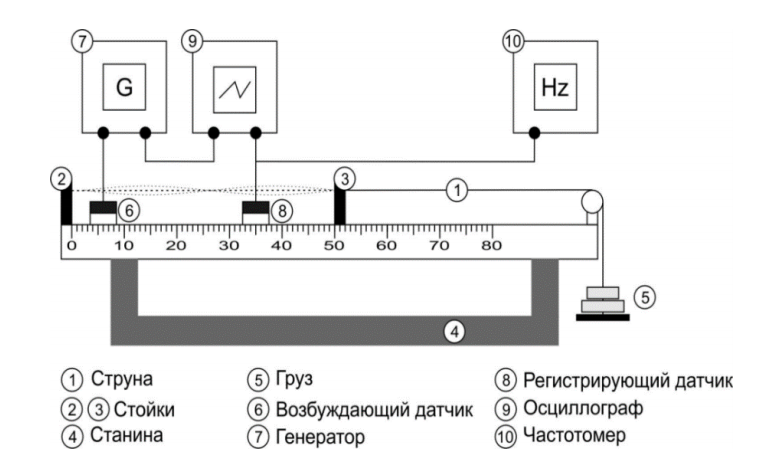
\includegraphics[width = 0.8\textwidth]{facility}
		\caption{Экспериментальная установка}
		\label{fig:facility}
	\end{center}
\end{figure}

На Рисунке \ref{fig:facility} представлена схема экспериментальной установки. Устроена она следующим образом: Стальная гитарная струна 1 закрепляется в горизонтальном положении между двумя стойками с зажимами 2 и 3,
расположенными на массивной станине 4. Один конец струны закреплен в
зажиме 2 неподвижно. К противоположному концу струны, перекинутому через блок, прикреплена платформа с грузами 5, создающими натяжение
струны. Зажим 3 можно передвигать по станине, устанавливая требуемую
длину струны. Возбуждение и регистрация колебаний струны осуществляются с помощью электромагнитных датчиков (вибраторов), расположенных
на станине под струной. Электромагнитный датчик 6 подключен к звуковому
генератору 7 и служит для возбуждения колебаний струны, частота которых
измеряется с помощью частотомера 10 (в некоторых установках частотомер
встроен в генератор). Колебания струны регистрируются с помощью электромагнитного датчика 8, сигнал с которого передается на вход осциллографа 9.
Разъёмы, через которые датчики с помощью кабелей соединяются с генератором и осциллографом, расположены на корпусе станины.



\section{Выполнение работы}


\subsection{Подготовка}
Мы работаем на установке №2. Освободим зажим на стойке 3, установим длинну струны $L=50$см. Натяним струну с помощью грузов (их массы занесем в таблицу \ref{tab:mass_of_load_for_all_measuring}). Расположим возбуждающий датчик 6 возле неподвижной стойки 2.

\begin{table}[h!]
\centering
\begin{tabular}{|c|c|c|c|c|c|c|c|c|c|}
\hline
Груз    & подвес   & кольцо     & платформа     & груз1     & груз2  & $\sum_{1}$  & груз3     & груз4   & $\sum_{2}$  \\ \hline
Масса груза $M,$ г & 108,1 & 1,175 & 106,9 & 493,2 & 493,4 &  12020,775 & 492,4 & 492,6 & 2187,775 \\ \hline
\end{tabular}
\caption{Масса грузов, используемых в ходе выполнения работы}
\label{tab:mass_of_load}
\end{table}


\subsection{Предварительные расчеты}
Оцените скорость распространения волн по формуле (\ref{eq:velocity_of_deformation}), используя табличное значение плотности стали и приняв диаметр струны равным $d\approx0,3$мм. Для заданных значений длины струны и силы натяжения рассчитаем частоту основной гармоники $\nu_{1}$ согласно (\ref{eq:frequency_velocity_equation}).\\
Получили $\nu_{1}=136,2 Hz$.


\subsection{Определение частоты первой гармоники по частотомеру}
Подключаем звуковой генератор и частотомер. Частоту устанавлием такую, как $\nu_{1}$ из предыдущего пункта, а амплитуду напряжения ставим максимальной. Частоту будем менять в пределах $\nu_{1}\pm5 Hz$


\subsection{Частоты на более высоких гармониках}
Пропорционально увеличивая частоту в $n$ раз мы получаем картину стоячих волн на n-ой гармонике. 


\subsection{Работа с осциллографом}
Проведем измерение частот не менее 5 нечетных ($n$ = 1, 3, 5, 7, 9) гармоник стоячих волн при длине струны 50 см и массе грузов $\approx1$кг. Для наблюдения нечетных гармоник регистрирующий датчик следует размещать в центре под струной (как для основной гармоники).\\


Измерим частоты четных ($n$ = 2, 4, …) гармоник.\\

По результатам этих измерений построим графики $\nu_{n}(n)$ для различных $T$. Определим скорости волн $n$ и оценим ее погрешность. Погрешности $\nu$ принимаем 0,2 Гц.

\begin{table}[h!]
\centering
\begin{tabular}{|c|c|c|c|c|c|c|}
\hline
№ измерения & 1        & 2        & 3        & 4        & 5        & 6        \\ \hline
$\nu_{1}$, Гц      & 132    & 136,2    & XXX    & XXX    & XXX    & XXX    \\ \hline
$\nu_{2}$, Гц      & 272,4    & 276    & XXX   & XXX      & XXX    & XXX    \\ \hline
$\nu_{3}$, Гц      & 408,6    & 413,2    & XXX    & XXX      & XXX    & XXX    \\ \hline
$\nu_{4}$, Гц      & 544    & 552    & XXX    & XXX    & XXX      & XXX    \\ \hline
$\nu_{5}$, Гц      & 681      & 690,4    & XXX    & XXX     & XXX     & XXX     \\ \hline
$\nu_{6}$, Гц      & XXX    & XXX     & XXX     & XXX   & XXX   & XXX   \\ \hline
$\nu_{7}$, Гц      & 953,4    & 971,5     & XXX   & XXX   & XXX   & XXX   \\ \hline
$\nu_{8}$, Гц      & XXX     & XXX  & 1525  & XXX & XXX & XXX \\ \hline
$\nu_{9}$, Гц      & 1224   & 1256 & 1713,5 & XXX & XXX & XXX \\ \hline
\end{tabular}
\caption{Результаты измерений частот гармоник в зависимости от массы нагрузки.}
\label{tab:measuring_results}
\end{table}
\newpage

\subsection{Фигуры Лиссажу}
Уменьшим частоту возбуждения в два раза, для нас это значение равно $\nu=\frac{\nu_{1}}{2}=95,7 Hz$. Фигура, появившаяся на экране осциллографа:


\subsection{Добротность}
Определим добротность $Q$ струны как колебательной системы, измерив её амплитудно-частотную характеристику (АЧХ) вблизи одной из резонансных частот ($\nu_{1}$ или $\nu_{3}$) для нескольких натяжений струны (по указанию преподавателя).
Для расчетов используем $Q=\frac{\nu_{resonance}}{\Delta\nu}$


\subsection{Ещё график}
Построим график зависимости $u^2(T)$. Определим погонную плотность $\rho_{l}$ струны и оценим погрешность результата. Сравним результаты с указанными на установке.


\section{Выводы}


\end{document}